%package list
\documentclass{article}
\usepackage[top=3cm, bottom=3cm, outer=3cm, inner=3cm]{geometry}
\usepackage{multicol}
\usepackage{graphicx}
\usepackage{url}
%\usepackage{cite}
\usepackage{hyperref}
\usepackage{array}
%\usepackage{multicol}
\newcolumntype{x}[1]{>{\centering\arraybackslash\hspace{0pt}}p{#1}}
\usepackage{natbib}
\usepackage{pdfpages}
\usepackage{multirow}
\usepackage[normalem]{ulem}
\useunder{\uline}{\ul}{}
\usepackage{svg}
\usepackage{xcolor}
\usepackage{listings}
\lstdefinestyle{ascii-tree}{
    literate={├}{|}1 {─}{--}1 {└}{+}1 
  }
\lstset{basicstyle=\ttfamily,
  showstringspaces=false,
  commentstyle=\color{red},
  keywordstyle=\color{blue}
}
%\usepackage{booktabs}
\usepackage{caption}
\usepackage{subcaption}
\usepackage{float}
\usepackage{array}

\newcolumntype{M}[1]{>{\centering\arraybackslash}m{#1}}
\newcolumntype{N}{@{}m{0pt}@{}}


%%%%%%%%%%%%%%%%%%%%%%%%%%%%%%%%%%%%%%%%%%%%%%%%%%%%%%%%%%%%%%%%%%%%%%%%%%%%
%%%%%%%%%%%%%%%%%%%%%%%%%%%%%%%%%%%%%%%%%%%%%%%%%%%%%%%%%%%%%%%%%%%%%%%%%%%%
\newcommand{\itemEmail}{rvaldiviase@unsa.edu.pe}
\newcommand{\itemStudent}{Ryan Fabian Valdivia Segovia}
\newcommand{\itemCourse}{Fundamentos de la programación 2}
\newcommand{\itemCourseCode}{1701213}
\newcommand{\itemSemester}{II}
\newcommand{\itemUniversity}{Universidad Nacional de San Agustín de Arequipa}
\newcommand{\itemFaculty}{Facultad de Ingeniería de Producción y Servicios}
\newcommand{\itemDepartment}{Departamento Académico de Ingeniería de Sistemas e Informática}
\newcommand{\itemSchool}{Escuela Profesional de Ingeniería de Sistemas}
\newcommand{\itemAcademic}{2023 - B}
\newcommand{\itemInput}{Del 18 Septiembre 2023}
\newcommand{\itemOutput}{Al 24 Septiembre 2023}
\newcommand{\itemPracticeNumber}{04}
\newcommand{\itemTheme}{Arreglos de objetos, Búsqueda y Algoritmos de ordenamiento}
%%%%%%%%%%%%%%%%%%%%%%%%%%%%%%%%%%%%%%%%%%%%%%%%%%%%%%%%%%%%%%%%%%%%%%%%%%%%
%%%%%%%%%%%%%%%%%%%%%%%%%%%%%%%%%%%%%%%%%%%%%%%%%%%%%%%%%%%%%%%%%%%%%%%%%%%%

\usepackage[english,spanish]{babel}
\usepackage[utf8]{inputenc}
\AtBeginDocument{\selectlanguage{spanish}}
\renewcommand{\figurename}{Figura}
\renewcommand{\refname}{Referencias}
\renewcommand{\tablename}{Tabla} %esto no funciona cuando se usa babel
\AtBeginDocument{%
	\renewcommand\tablename{Tabla}
}

\usepackage{fancyhdr}
\pagestyle{fancy}
\fancyhf{}
\setlength{\headheight}{30pt}
\renewcommand{\headrulewidth}{1pt}
\renewcommand{\footrulewidth}{1pt}
\fancyhead[L]{\raisebox{-0.2\height}{
\includegraphics[width=3cm]{img/logo_episunsa.png}}}
\fancyhead[C]{\fontsize{7}{7}\selectfont	\itemUniversity \\ \itemFaculty \\ \itemDepartment \\ \itemSchool \\ \textbf{\itemCourse}}
\fancyhead[R]{\raisebox{-0.2\height}{
\includegraphics[width=1.2cm]{img/logo_abet}}}
\fancyfoot[L]{Estudiante Ryan Valdivia}
\fancyfoot[C]{\itemCourse}
\fancyfoot[R]{Página \thepage}

% para el codigo fuente
\usepackage{listings}
\usepackage{color, colortbl}
\definecolor{dkgreen}{rgb}{0,0.6,0}
\definecolor{gray}{rgb}{0.5,0.5,0.5}
\definecolor{mauve}{rgb}{0.58,0,0.82}
\definecolor{codebackground}{rgb}{0.95, 0.95, 0.92}
\definecolor{tablebackground}{rgb}{0.8, 0, 0}

\lstset{frame=tb,
	language=bash,
	aboveskip=3mm,
	belowskip=3mm,
	showstringspaces=false,
	columns=flexible,
	basicstyle={\small\ttfamily},
	numbers=none,
	numberstyle=\tiny\color{gray},
	keywordstyle=\color{blue},
	commentstyle=\color{dkgreen},
	stringstyle=\color{mauve},
	breaklines=true,
	breakatwhitespace=true,
	tabsize=3,
	backgroundcolor= \color{codebackground},
}

\begin{document}
	
	\vspace*{10px}
	
	\begin{center}	
		\fontsize{17}{17} \textbf{ Informe de Laboratorio \itemPracticeNumber}
	\end{center}
	\centerline{\textbf{\Large Tema: \itemTheme}}
	%\vspace*{0.5cm}	

	\begin{flushright}
		\begin{tabular}{|M{2.5cm}|N|}
			\hline 
			\rowcolor{tablebackground}
			\color{white} \textbf{Nota}  \\
			\hline 
			     \\[30pt]
			\hline 			
		\end{tabular}
	\end{flushright}	

	\begin{table}[H]
		\begin{tabular}{|x{4.7cm}|x{4.8cm}|x{4.8cm}|}
			\hline 
			\rowcolor{tablebackground}
			\color{white} \textbf{Estudiante} & \color{white}\textbf{Escuela}  & \color{white}\textbf{Asignatura}   \\
			\hline 
			{\itemStudent \par \itemEmail} & \itemSchool & {\itemCourse \par Semestre: \itemSemester \par Código: \itemCourseCode}     \\
			\hline 			
		\end{tabular}
	\end{table}		
	
	\begin{table}[H]
		\begin{tabular}{|x{4.7cm}|x{4.8cm}|x{4.8cm}|}
			\hline 
			\rowcolor{tablebackground}
			\color{white}\textbf{Laboratorio} & \color{white}\textbf{Tema}  & \color{white}\textbf{Duración}   \\
			\hline 
			\itemPracticeNumber & \itemTheme & 04 horas   \\
			\hline 
		\end{tabular}
	\end{table}
	
	\begin{table}[H]
		\begin{tabular}{|x{4.7cm}|x{4.8cm}|x{4.8cm}|}
			\hline 
			\rowcolor{tablebackground}
			\color{white}\textbf{Semestre académico} & \color{white}\textbf{Fecha de inicio}  & \color{white}\textbf{Fecha de entrega}   \\
			\hline 
			\itemAcademic & \itemInput &  \itemOutput  \\
			\hline 
		\end{tabular}
	\end{table}
	
	\section{Tarea}
	\begin{itemize}
		\subsection{Actividad: Demo Batalla}
			\item Analice, complete y pruebe el Código de la clase DemoBatalla.
	\end{itemize}
		
	\section{Equipos, materiales y temas utilizados}
	\begin{itemize}
		\item Sistema Operativo Windows 11 Home Single Language 64 bits 22621.2283
		\item VIM 9.0.
		\item Visual Studio Code 64 bits 1.82.2
		\item OpenJDK 64-Bits 11.0.16.1
		\item Git 2.41.0.windows.1
		\item Cuenta en GitHub con el correo institucional. 
		\item Código parcial proporcionado por el profesor.
	\end{itemize}
	
	\section{URL de Repositorio Github}
	\begin{itemize}
		\item URL del Repositorio GitHub para clonar o recuperar.
		\item \url{https://github.com/RyanValdivia/fp2-23b.git}
		\item URL para el laboratorio 04 en el Repositorio GitHub.
		\item \url{https://github.com/RyanValdivia/fp2-23b/tree/main/fase01/lab04}
	\end{itemize}
	
	\section{Actividades}
	\subsection{Actividad 1}
	
	\begin{itemize}	
		\item Realicé un commit reutilizando el código ya hecho del laboratorio anterior.
	\end{itemize}	
	\begin{lstlisting}[language=bash,caption={Comentando el código parcial}][H]
		$ git log Ahorcado.java
		commit d44ccee0c41e9bfcd80323582d0cea9defa7667b
		Author: RYAN VALDIVIA <rvaldiviase@unsa.edu.pe>
		Date:   Wed Sep 27 16:18:18 2023 -0500
			Reutilizando el codigo del laboratorio anterior
	\end{lstlisting}
	\begin{itemize}	
		\item Lo primero que hice fue elaborar el método para intercambiar los valores en el arreglo, algo muy utilizado en los métodos de ordenamiento.
	\end{itemize}
	\begin{lstlisting}[language=java,caption={Intercambio}, numbers=left][H]
	public static void intercambiar(Nave[] flota, int i, int j) {
        Nave temp;
        temp = flota[i];
        flota[i] = flota[j];
        flota[j] = temp;
    }
	\end{lstlisting}
	\begin{itemize}	
		\item Seguidamente, comencé elaborando los métodos de ordenamiento, ya que para realizar búsqueda binaria en un arreglo, debe estar ordenado.
		\item Comencé con el ordenamiento por burbuja, realizando sus dos variantes, uno para datos enteros (el puntaje de las naves) y otro para Strings (los nombres).
	\end{itemize}
	\begin{lstlisting}[language=java,caption={Ordenamiento por burbuja: Enteros}, numbers=left][H]
	public static void ordenarPorPuntosBurbuja(Nave[] flota) {
        for (int i = 0; i < flota.length; i++) {
            for (int j = 0; j < flota.length - 1; j++) {
                if (flota[j].getPuntos() > flota[j + 1].getPuntos()) {
                    intercambiar(flota, j, j + 1);
                }
            }
        }
    }
	\end{lstlisting}
	\begin{itemize}	
		\item En este algoritmo se intercambian valores de dos en dos para ordenar el arreglo.
		\item Este es un método conocido para ordenar, la variante se presenta con las cadenas o strings, donde en lugar de ir comparando los valores, uso el método compareTo() para ir comparando sus valores alfabéticos e irlos ordenando.
	\end{itemize}
	\begin{lstlisting}[language=java,caption={Ordenamiento por burbuja: Cadenas}, numbers=left][H]
	public static void ordenarPorNombreBurbuja(Nave[] flota) {
        for (int i = 0; i < flota.length; i++) {
            for (int j = 0; j < flota.length - 1; j++) {
                if (flota[j].getNombre().compareTo(flota[j + 1].getNombre()) > 0) {
                    intercambiar(flota, j, j + 1);
                }
            }
        }
    }
	\end{lstlisting}
	\begin{itemize}	
		\item Una vez que ya tenía hecho un par de métodos de ordenamiento, procedí a la búsqueda binaria. La realicé para buscar un nombre dentro de una lista ordenada.
	\end{itemize}
	\begin{lstlisting}[language=java,caption={Búsqueda binaria: Cadenas}, numbers=left][H]
	public static int busquedaBinariaNombre(Nave[] flota, String s) {
        int baja = 0, media, alta = flota.length - 1;
        while (baja <= alta) {
            media = (alta + baja) / 2;
            String nMedio = flota[media].getNombre();
            int compare = s.compareTo(nMedio);
            if (compare == 0) {
                return media;
            } else if (compare < 0) {
                alta = media - 1;
            } else {
                baja = media + 1;
            }
        }
        return -1;
    }
	\end{lstlisting}	
	\begin{itemize}	
		\item Además, cree un método para la búsqueda lineal en un arreglo (No necesita estar ordenado).
	\end{itemize}
	\begin{lstlisting}[language=java,caption={Método para obtener números desordenados}, numbers=left][H]
	 public static int busquedaLinealNombre(Nave[] flota, String s) {
        for (int i = 0; i < flota.length; i++) {
            if (flota[i].getNombre().equals(s)) {
                return i;
            }
        }
        return -1;
    }
	\end{lstlisting}
	\begin{itemize}	
		\item Asímismo, creé el resto de métodos de ordenamiento, como el de selección.
		\item Realicé dos variantes, una para la búsqueda de valores enteros (Puntaje) y para cadenas (Nombres) utilizando compareTo de nuevo para obtener el menor valor alfabético del arreglo.
	\end{itemize}
	\begin{lstlisting}[language=java,caption={Ordenamiento por selección: Enteros}, numbers=left][H]
	 public static void ordenarPorPuntosSeleccion(Nave[] flota) {
        for (int i = 0; i < flota.length - 1; i++) {
            int menor = flota[i].getPuntos();
            int indice = i;
            for (int j = i + 1; j < flota.length; j++) {
                if (flota[j].getPuntos() < menor) {
                    menor = flota[j].getPuntos();
                    indice = j;
                }
            }
            if (indice != i) {
                Nave pivot = flota[i];
                flota[i] = flota[indice];
                flota[indice] = pivot;
            }
        }
    }
	\end{lstlisting}
	\begin{itemize}	
		\item Para este algoritmo, se parte del primer elemento del arreglo y se selecciona el menor valor de todo el arreglo, si este es menor que nuestro valor inicial, se intercambian, y asi seguimos intercambiando hasta que la lista esté ordenada.
	\end{itemize}
	\begin{lstlisting}[language=java,caption={Ordenamiento por selección: Cadenas}, numbers=left][H]
	 public static void ordenarPorNombreSeleccion(Nave[] flota) {
        for (int i = 0; i < flota.length - 1; i++) {
            String menor = flota[i].getNombre();
            int indice = i;
            for (int j = i + 1; j < flota.length; j++) {
                if (flota[i].getNombre().compareTo(menor) < 0) {
                    menor = flota[j].getNombre();
                    indice = j;
                }
            }
            if (indice != i) {
                Nave pivot = flota[i];
                flota[i] = flota[indice];
                flota[indice] = pivot;
            }
        }
    }
	\end{lstlisting}
	\begin{itemize}	
		\item Ahora sigue los algoritmos de ordenamiento por inserción, también dos variantes. Una para números enteros (el puntaje) y otra para los nombres, sin embargo. Ahora una variación más es para ordenar los nombres de la Z a la A, en vez de al revés como he estado haciendo hasta ahora.
	\end{itemize}
	\begin{lstlisting}[language=java,caption={Ordenamiento por inserción: Enteros}, numbers=left][H]
	 public static void ordenarPorPuntosInsercion(Nave[] flota) {
        for (int i = 1; i < flota.length; i++) {
            Nave valor = flota[i];
            int j = i;
            for (j = i; 0 < j && flota[j - 1].getPuntos() > valor.getPuntos(); j--) {
                flota[j] = flota[j - 1];
            }
            flota[j] = valor;
        }

    }
	\end{lstlisting}
	\begin{itemize}	
		\item La lógica es, dado una lista desordenada, se parte desde el segundo término y se compara los valores hacia la izquierda, si es mayor el valor a la izquierda, se inserta hacia esa dirección hasta que toda la lista este ordenada.
	\end{itemize}
	\begin{lstlisting}[language=java,caption={Ordenamiento por inserción: Cadenas de la Z a la A}, numbers=left][H]
	 public static void ordenarPorNombreInsercion(Nave[] flota) {
        for (int i = 1; i < flota.length; i++) {
            Nave valor = flota[i];
            int j = i;
            for (j = i; 0 < j && flota[j - 1].getNombre().compareTo(valor.getNombre()) < 0; j--) {
                flota[j] = flota[j - 1];
            }
            flota[j] = valor;
        }
    }
	\end{lstlisting}
	\begin{itemize}	
		\item Solo que en este caso, hacemos una modificación para que los valores mayores queden a la izquierda, ya que queremos que la lista esté ordenada de la Z a la A.
		\item Con esto ya tenemos algoritmos hechos para poder ordenar y buscar en arreglos.
	\end{itemize}
	\begin{lstlisting}[language=java,caption={Aplicando los métodos de búsqueda}, numbers=left][H]
	 	int pos = busquedaLinealNombre(misNaves, nombre);
        if (pos != -1) {
            Nave n = misNaves[pos];
            System.out.println("Nave " + pos + ":" + n.getNombre());
            System.out.println("Posicion: " + n.getFila() + n.getColumna());
            System.out.println("Puntos: " + n.getPuntos());
            if (n.getEstado()) {
                System.out.println("Sigue con vida");
            } else {
                System.out.println("Fue destruida");
            }
        } else {
            System.out.println("Nave no encontrada");
        }
        ordenarPorPuntosBurbuja(misNaves);
	\end{lstlisting}
	\begin{itemize}	
		\item A continuación pruebo el código con cinco naves para no tener que ingresar tantos datos.
	\end{itemize}
	\begin{lstlisting}[language=bash,caption={Prueba del código}][H]
	 $javac DemoBatalla.java Nave.java
	 $java DemoBatalla
	 Nave 1:
	 Connor 1 A true 60
	 Nave 2:
	 Delta 3 C true 25
	 Nave 3:
	 Whisky 6 J true 40
	 Nave 4:
	 Jayce 7 A true 55
	 Nave 5:
	 Abigail 8 B true 42
	\end{lstlisting}
	
	\begin{figure}[H]
		\centering
		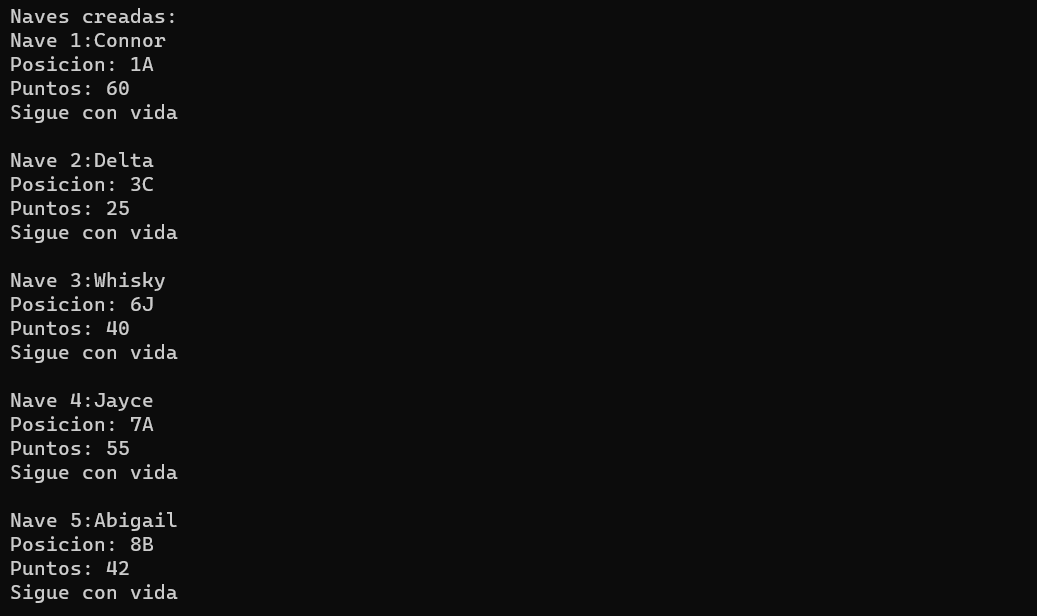
\includegraphics[width=0.8\textwidth,keepaspectratio]{img/captura1.png}
		%\includesvg{img/automata.svg}
		%\label{img:mot2}
		%\caption{Product backlog.}
	\end{figure}
	\begin{itemize}
		\item Mostrando las naves.
	\end{itemize}
	
	\begin{figure}[H]
		\centering
		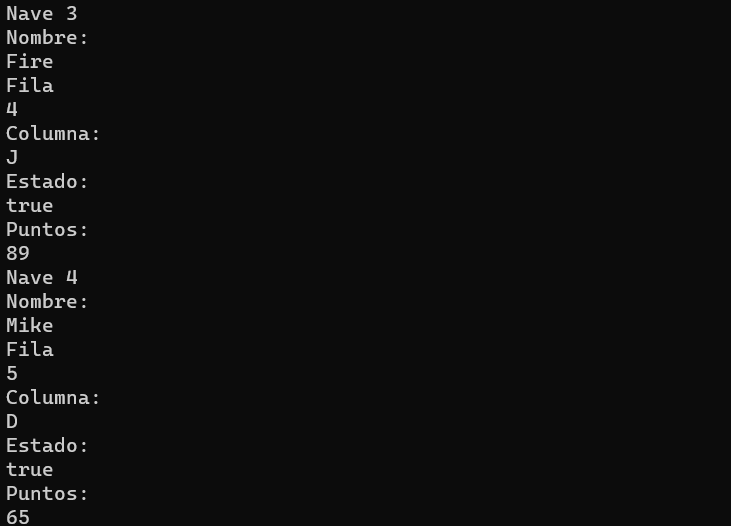
\includegraphics[width=0.8\textwidth,keepaspectratio]{img/captura2.png}
		%\includesvg{img/automata.svg}
		%\label{img:mot2}
		%\caption{Product backlog.}
	\end{figure}
	\begin{itemize}
		\item Buscando un nombre.
	\end{itemize}
	
	\begin{figure}[H]
		\centering
		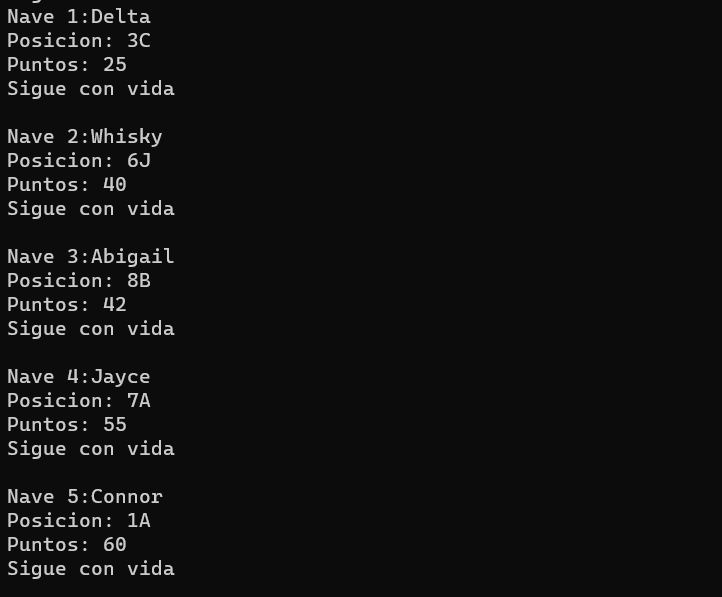
\includegraphics[width=0.8\textwidth,keepaspectratio]{img/captura3.png}
		%\includesvg{img/automata.svg}
		%\label{img:mot2}
		%\caption{Product backlog.}
	\end{figure}
	\begin{itemize}
		\item Ordenando por puntaje.
	\end{itemize}
	
	\begin{figure}[H]
		\centering
		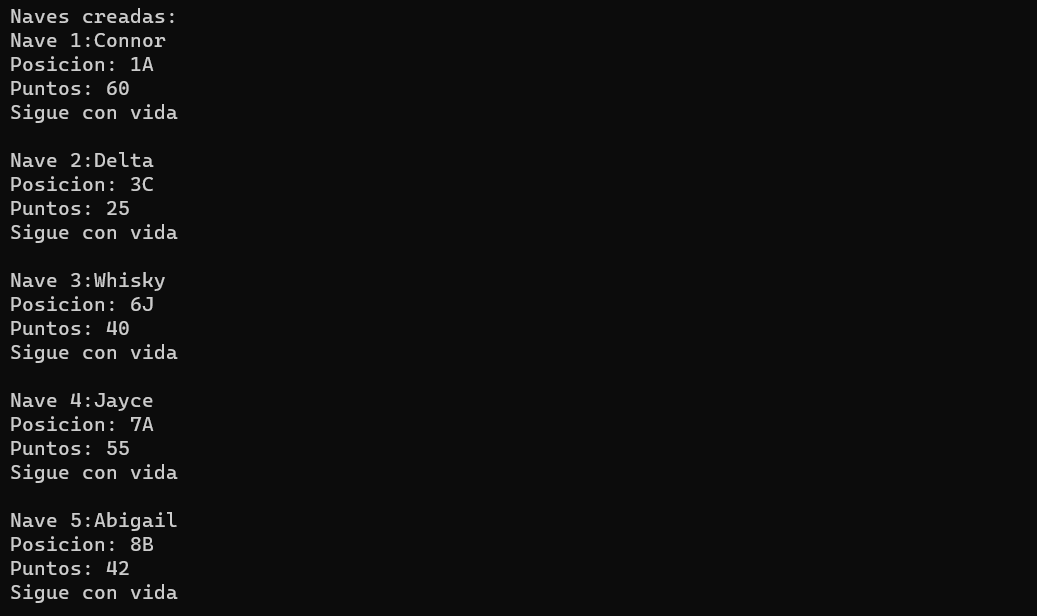
\includegraphics[width=0.8\textwidth,keepaspectratio]{img/captura1.png}
		%\includesvg{img/automata.svg}
		%\label{img:mot2}
		%\caption{Product backlog.}
	\end{figure}
	\begin{itemize}
		\item Ordenando por nombre.
	\end{itemize}
	
	\section{\textcolor{red}{Rúbricas}}
	
	\subsection{\textcolor{red}{Entregable Informe}}
	\begin{table}[H]
		\caption{Tipo de Informe}
		\setlength{\tabcolsep}{0.5em} % for the horizontal padding
		{\renewcommand{\arraystretch}{1.5}% for the vertical padding
		\begin{tabular}{|p{3cm}|p{12cm}|}
			\hline
			\multicolumn{2}{|c|}{\textbf{\textcolor{red}{Informe}}}  \\
			\hline 
			\textbf{\textcolor{red}{Latex}} & \textcolor{blue}{El informe está en formato PDF desde Latex,  con un formato limpio (buena presentación) y facil de leer.}   \\ 
			\hline 
			
			
		\end{tabular}
	}
	\end{table}
	
	\clearpage
	
	\subsection{\textcolor{red}{Rúbrica para el contenido del Informe y demostración}}
	\begin{itemize}			
		\item El alumno debe marcar o dejar en blanco en celdas de la columna \textbf{Checklist} si cumplio con el ítem correspondiente.
		\item Si un alumno supera la fecha de entrega,  su calificación será sobre la nota mínima aprobada, siempre y cuando cumpla con todos lo items.
		\item El alumno debe autocalificarse en la columna \textbf{Estudiante} de acuerdo a la siguiente tabla:
	
		\begin{table}[ht]
			\caption{Niveles de desempeño}
			\begin{center}
			\begin{tabular}{ccccc}
    			\hline
    			 & \multicolumn{4}{c}{Nivel}\\
    			\cline{1-5}
    			\textbf{Puntos} & Insatisfactorio 25\%& En Proceso 50\% & Satisfactorio 75\% & Sobresaliente 100\%\\
    			\textbf{2.0}&0.5&1.0&1.5&2.0\\
    			\textbf{4.0}&1.0&2.0&3.0&4.0\\
    		\hline
			\end{tabular}
		\end{center}
	\end{table}	
	
	\end{itemize}
	
	\begin{table}[H]
		\caption{Rúbrica para contenido del Informe y demostración}
		\setlength{\tabcolsep}{0.5em} % for the horizontal padding
		{\renewcommand{\arraystretch}{1.5}% for the vertical padding
		%\begin{center}
		\begin{tabular}{|p{2.7cm}|p{7cm}|x{1.3cm}|p{1.2cm}|p{1.5cm}|p{1.1cm}|}
			\hline
    		\multicolumn{2}{|c|}{Contenido y demostración} & Puntos & Checklist & Estudiante & Profesor\\
			\hline
			\textbf{1. GitHub} & Hay enlace URL activo del directorio para el  laboratorio hacia su repositorio GitHub con código fuente terminado y fácil de revisar. &2 &X &2 & \\ 
			\hline
			\textbf{2. Commits} &  Hay capturas de pantalla de los commits más importantes con sus explicaciones detalladas. (El profesor puede preguntar para refrendar calificación). &4 &X &2 & \\ 
			\hline 
			\textbf{3. Código fuente} &  Hay porciones de código fuente importantes con numeración y explicaciones detalladas de sus funciones. &2 &X &2 & \\ 
			\hline 
			\textbf{4. Ejecución} & Se incluyen ejecuciones/pruebas del código fuente  explicadas gradualmente. &2 &X &2 & \\ 
			\hline			
			\textbf{5. Pregunta} & Se responde con completitud a la pregunta formulada en la tarea.  (El profesor puede preguntar para refrendar calificación).  &2 &X &2 & \\ 
			\hline	
			\textbf{6. Fechas} & Las fechas de modificación del código fuente estan dentro de los plazos de fecha de entrega establecidos. &2 &X &2 & \\ 
			\hline 
			\textbf{7. Ortografía} & El documento no muestra errores ortográficos. &2 &X &2 & \\ 
			\hline 
			\textbf{8. Madurez} & El Informe muestra de manera general una evolución de la madurez del código fuente,  explicaciones puntuales pero precisas y un acabado impecable.   (El profesor puede preguntar para refrendar calificación).  &4 &X &4 & \\ 
			\hline
			\multicolumn{2}{|c|}{\textbf{Total}} &20 & &18 & \\ 
			\hline
		\end{tabular}
		%\end{center}
		%\label{tab:multicol}
		}
	\end{table}
	
\clearpage

\section{Referencias}
	\begin{itemize}
		\item Fundamentos de la programación 2 - Tópicos de la programación Orientada a Objetos (Marco Aedo)
	\end{itemize}
	
%\clearpage
%\bibliographystyle{apalike}
%\bibliographystyle{IEEEtranN}
%\bibliography{bibliography}
			
\end{document}
